\begin{center}
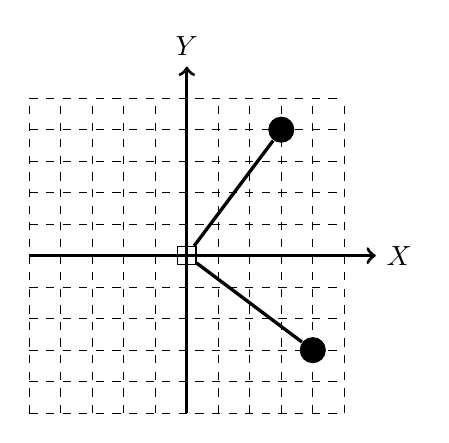
\begin{tikzpicture}[scale=0.4]

\draw[dashed] (-5, -5) grid (5, 5);

\draw[very thick, ->] (-5, 0) -- (6, 0) node[right]{$X$};
\draw[very thick, ->] (0, -5) -- (0, 6) node[above]{$Y$};

\node[circle, fill=black] (1) at (3, 4) {};
\node[circle, fill=black] (2) at (4, -3) {};
\node[rectangle, draw=black] (0) at (0, 0) {};

\draw[very thick] (0) -- (1);
\draw[very thick] (0) -- (2);

\end{tikzpicture}
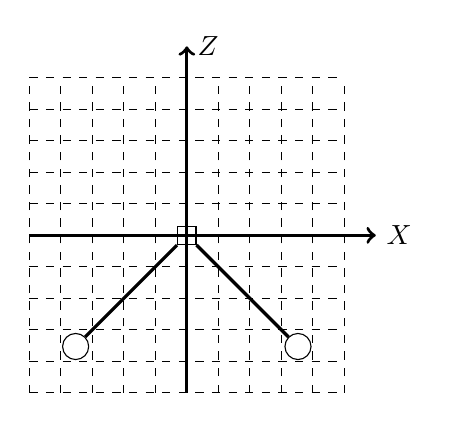
\begin{tikzpicture}[scale=0.4]

\draw[dashed] (-5, -5) grid (5, 5);

\draw[very thick, ->] (-5, 0) -- (6, 0) node[right]{$X$};
\draw[very thick, ->] (0, -5) -- (0, 6) node[right]{$Z$};

\node[rectangle, draw=black] (0) at (0, 0) {};
\node[circle, draw=black] (3) at (3.53, -3.53) {};
\node[circle, draw=black] (4) at (-3.53, -3.53) {};

\draw[very thick] (0) -- (3);
\draw[very thick] (0) -- (4);

\end{tikzpicture}
\end{center}
